You can write monospace letters \texttt{like that}.

You can create itemization like that:
\begin{itemize}
	\item Example item 1
	\item Example item 2
	\begin{itemize}
		\item Example subitem 1
		\item Example subitem 2
	\end{itemize}
	\item Example item 3
\end{itemize}

You can cite like that:
\cite{torvalds2001just,kopka2004guide,yakaryilmaz2011unbounded,bernstein2019fast}

If you need to give reference number, you can cite like that:
ref~\citenum{almheiri2021entropy}

You can create a table like that:
\begin{table}[H]
	\centering
	\caption{An example table made up of 3 rows and 3 columns. Resizebox is used to scale relatively wide tables.}
    \resizebox{0.5\linewidth}{!}{
		\begin{tabular}{|c|c|c|}
			\hline
			\textbf{Col 1} & \textbf{Col 2} & \textbf{Col 3} \\
			\hline
			Example 1.1 & Example 2.1 & Example 3.1 \\
			\hline
			Example 2.1 & Example 2.2 & Example 2.3 \\
			\hline
		\end{tabular}
	}
	\label{tab:example}
\end{table}
Also, you can refere a table like that: "Table \ref{tab:example}".

\blindtext[1]

You can create a figure like that:
\begin{figure}[H]
    \centering
	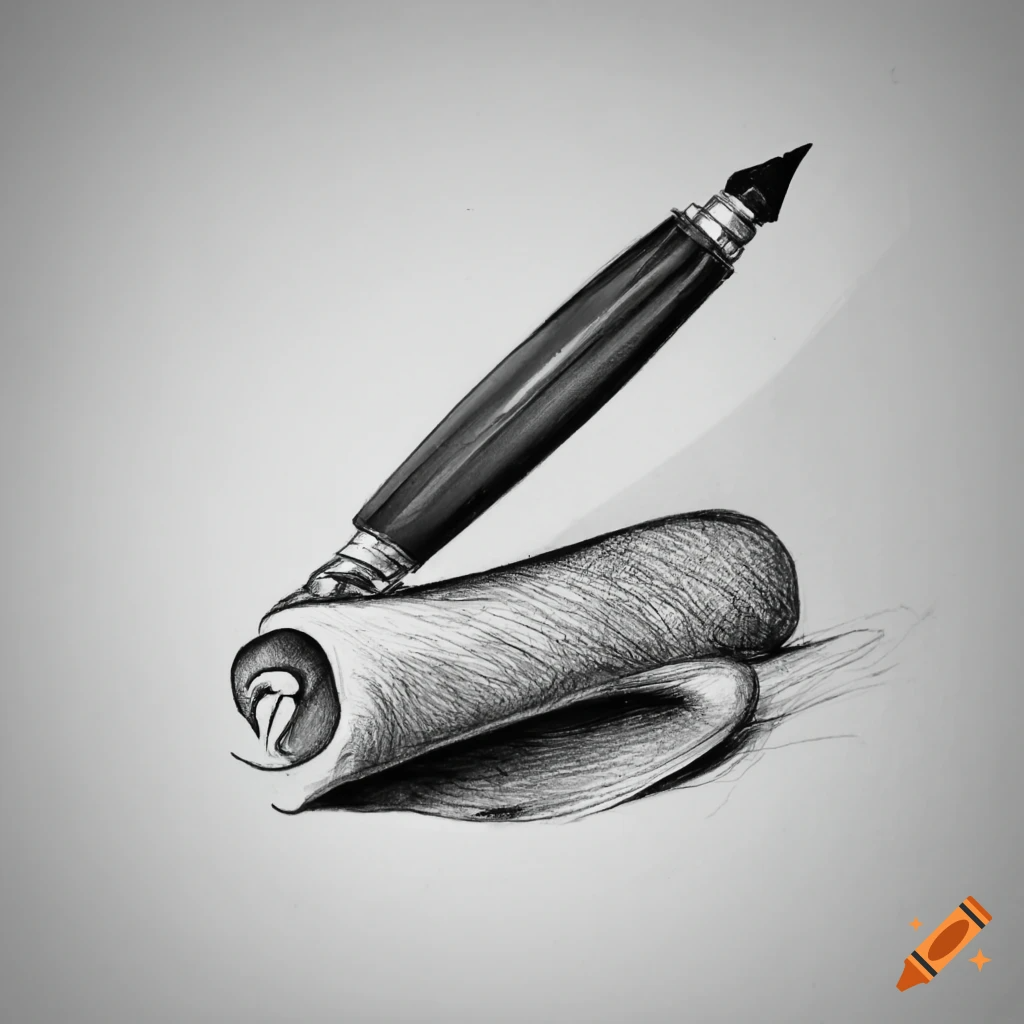
\includegraphics[width=0.5\textwidth]{chapters/images/example-figure.png}
	\caption{The image is a black-and-white pencil sketch showing a pen appearing to be writing on a rolled-up piece of paper. The style is realistic but slightly stylized, emphasizing texture and form.}
	\label{fig:example}
\end{figure}
Also, you can refere a figure like that: "Figure \ref{fig:example}".

\blindtext[1]
